\section{mo\-Sol\-Continue$<$ EOT $>$ Class Template Reference}
\label{classmo_sol_continue}\index{moSolContinue@{moSolContinue}}
Class that describes a stop criterion for a solution-based heuristic.  


{\tt \#include $<$mo\-Sol\-Continue.h$>$}

Inheritance diagram for mo\-Sol\-Continue$<$ EOT $>$::\begin{figure}[H]
\begin{center}
\leavevmode
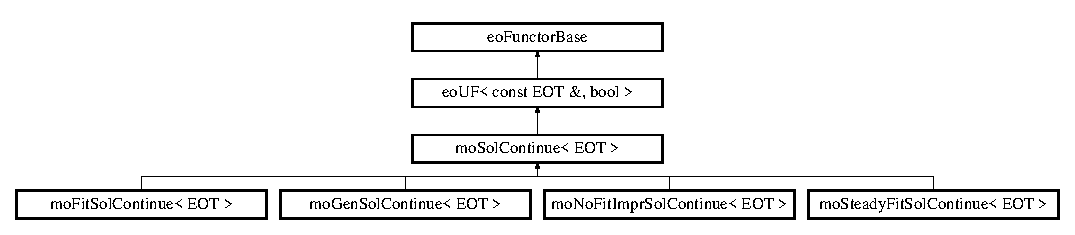
\includegraphics[height=2.70531cm]{classmo_sol_continue}
\end{center}
\end{figure}
\subsection*{Public Member Functions}
\begin{CompactItemize}
\item 
virtual void {\bf init} ()=0
\begin{CompactList}\small\item\em Procedure which initialises all that the stop criterion needs. \item\end{CompactList}\end{CompactItemize}


\subsection{Detailed Description}
\subsubsection*{template$<$class EOT$>$ class mo\-Sol\-Continue$<$ EOT $>$}

Class that describes a stop criterion for a solution-based heuristic. 

It allows to add an initialisation procedure to an object that is a unary function ({\bf eo\-UF}). 



Definition at line 48 of file mo\-Sol\-Continue.h.

\subsection{Member Function Documentation}
\index{moSolContinue@{mo\-Sol\-Continue}!init@{init}}
\index{init@{init}!moSolContinue@{mo\-Sol\-Continue}}
\subsubsection{\setlength{\rightskip}{0pt plus 5cm}template$<$class EOT$>$ virtual void {\bf mo\-Sol\-Continue}$<$ EOT $>$::init ()\hspace{0.3cm}{\tt  [pure virtual]}}\label{classmo_sol_continue_a0}


Procedure which initialises all that the stop criterion needs. 

Generally, it allocates some data structures or initialises some counters. 

Implemented in {\bf mo\-Fit\-Sol\-Continue$<$ EOT $>$} {\rm (p.\,\pageref{classmo_fit_sol_continue_a2})}, {\bf mo\-Gen\-Sol\-Continue$<$ EOT $>$} {\rm (p.\,\pageref{classmo_gen_sol_continue_a2})}, {\bf mo\-No\-Fit\-Impr\-Sol\-Continue$<$ EOT $>$} {\rm (p.\,\pageref{classmo_no_fit_impr_sol_continue_a2})}, and {\bf mo\-Steady\-Fit\-Sol\-Continue$<$ EOT $>$} {\rm (p.\,\pageref{classmo_steady_fit_sol_continue_a2})}.

The documentation for this class was generated from the following file:\begin{CompactItemize}
\item 
mo\-Sol\-Continue.h\end{CompactItemize}
